% This is "aamas2017_sample.tex", a revised version of aamas2016_sample.tex
% This file should be compiled with "aamas2017.cls"
% This example file demonstrates the use of the 'aamas2017.cls'
% LaTeX2e document class file. It is intended for those submitting
% articles to the AAMAS-2017 conference. This file is based on
% the sig-alternate.tex example file.
% The 'sig-alternate.cls' file of ACM will produce a similar-looking,
% albeit, 'tighter' paper resulting in, invariably, fewer pages
% than the original ACM style.
%
% ----------------------------------------------------------------------------------------------------------------
% This .tex file (and associated .cls ) produces:
%       1) The Permission Statement
%       2) The Conference (location) Info information
%       3) The Copyright Line with AAMAS data
%       4) NO page numbers
%
% as against the acm_proc_article-sp.cls file which
% DOES NOT produce 1) through 3) above.
%
% Using 'aamas2017.cls' you don't have control
% from within the source .tex file, over both the CopyrightYear
% (defaulted to 20XX) and the IFAAMAS Copyright Data
% (defaulted to X-XXXXX-XX-X/XX/XX).
% These information will be overwritten by fixed AAMAS 2017  information
% in the style files - it is NOT as you are used to with ACM style files.
%
% ---------------------------------------------------------------------------------------------------------------
% This .tex source is an example which *does* use
% the .bib file (from which the .bbl file is produced).
% REMEMBER HOWEVER: After having produced the .bbl file,
% and prior to final submission, you *NEED* to 'insert'
% your .bbl file into your source .tex file so as to provide
% ONE 'self-contained' source file.
%


\documentclass{aamas2017}

\usepackage[table,usenames,dvipsnames]{xcolor}
\usepackage[]{algorithm2e}

% if you are using PDF LaTeX and you cannot find a way for producing
% letter, the following explicit settings may help

\pdfpagewidth=8.5truein
\pdfpageheight=11truein

\begin{document}

% In the original styles from ACM, you would have needed to
% add meta-info here. This is not necessary for AAMAS 2017  as
% the complete copyright information is generated by the cls-files.


\title{From Misunderstanding to Cooperation: Understanding and Expressing Intentions Through Non-Communicative Actions}

% AUTHORS


% For initial submission, do not give author names, but the
% tracking number, instead, as the review process is blind.

% You need the command \numberofauthors to handle the 'placement
% and alignment' of the authors beneath the title.
%
% For aesthetic reasons, we recommend 'three authors at a time'
% i.e. three 'name/affiliation blocks' be placed beneath the title.
%
% NOTE: You are NOT restricted in how many 'rows' of
% "name/affiliations" may appear. We just ask that you restrict
% the number of 'columns' to three.
%
% Because of the available 'opening page real-estate'
% we ask you to refrain from putting more than six authors
% (two rows with three columns) beneath the article title.
% More than six makes the first-page appear very cluttered indeed.
%
% Use the \alignauthor commands to handle the names
% and affiliations for an 'aesthetic maximum' of six authors.
% Add names, affiliations, addresses for
% the seventh etc. author(s) as the argument for the
% \additionalauthors command.
% These 'additional authors' will be output/set for you
% without further effort on your part as the last section in
% the body of your article BEFORE References or any Appendices.

%\numberofauthors{8} %  in this sample file, there are a *total*
% of EIGHT authors. SIX appear on the 'first-page' (for formatting
% reasons) and the remaining two appear in the \additionalauthors section.
%

\numberofauthors{1}

\author{
% You can go ahead and credit any number of authors here,
% e.g. one 'row of three' or two rows (consisting of one row of three
% and a second row of one, two or three).
%
% The command \alignauthor (no curly braces needed) should
% precede each author name, affiliation/snail-mail address and
% e-mail address. Additionally, tag each line of
% affiliation/address with \affaddr, and tag the
% e-mail address with \email.
% 1st. author
\alignauthor
\# \# \#
%Ben Trovato\titlenote{Dr.~Trovato insisted his name be first.}\\
%       \affaddr{Institute for Clarity in Documentation}\\
%       \affaddr{1932 Wallamaloo Lane}\\
%       \affaddr{Wallamaloo, New Zealand}\\
%       \email{trovato@corporation.com}
% 2nd. author
%\alignauthor
%G.K.M. Tobin\titlenote{The secretary disavows any knowledge of this author's actions.}\\
%       \affaddr{Institute for Clarity in Documentation}\\
%       \affaddr{P.O. Box 1212}\\
%       \affaddr{Dublin, Ohio 43017-6221}\\
%       \email{webmaster@marysville-ohio.com}
% 3rd. author
%\alignauthor Lars Th{\o}rv{\"a}ld\titlenote{This author is the one who did all the really hard work.}\\
%       \affaddr{The Th{\o}rv{\"a}ld Group}\\
%       \affaddr{1 Th{\o}rv{\"a}ld Circle}\\
%       \affaddr{Hekla, Iceland}\\
%       \email{larst@affiliation.org}
}

%\and  % use '\and' if you need 'another row' of author names

% 4th. author
%\alignauthor Lawrence P. Leipuner\\
%       \affaddr{Brookhaven Laboratories}\\
%       \affaddr{Brookhaven National Lab}\\
%       \affaddr{P.O. Box 5000}\\
%       \email{lleipuner@researchlabs.org}

% 5th. author
%\alignauthor Sean Fogarty\\
%       \affaddr{NASA Ames Research Center}\\
%       \affaddr{Moffett Field}\\
%       \affaddr{California 94035}\\
%       \email{fogartys@amesres.org}

% 6th. author
%\alignauthor Charles Palmer\\
%       \affaddr{Palmer Research Laboratories}\\
%      \affaddr{8600 Datapoint Drive}\\
%       \affaddr{San Antonio, Texas 78229}\\
%       \email{cpalmer@prl.com}

%\and

%% 7th. author
%\alignauthor Lawrence P. Leipuner\\
%       \affaddr{Brookhaven Laboratories}\\
%       \affaddr{Brookhaven National Lab}\\
%       \affaddr{P.O. Box 5000}\\
%       \email{lleipuner@researchlabs.org}

%% 8th. author
%\alignauthor Sean Fogarty\\
%       \affaddr{NASA Ames Research Center}\\
%       \affaddr{Moffett Field}\\
%       \affaddr{California 94035}\\
%       \email{fogartys@amesres.org}

%% 9th. author
%\alignauthor Charles Palmer\\
%       \affaddr{Palmer Research Laboratories}\\
%       \affaddr{8600 Datapoint Drive}\\
%       \affaddr{San Antonio, Texas 78229}\\
%       \email{cpalmer@prl.com}

%}

%% There's nothing stopping you putting the seventh, eighth, etc.
%% author on the opening page (as the 'third row') but we ask,
%% for aesthetic reasons that you place these 'additional authors'
%% in the \additional authors block, viz.
%\additionalauthors{Additional authors: John Smith (The Th{\o}rv{\"a}ld Group,
%email: {\texttt{jsmith@affiliation.org}}) and Julius P.~Kumquat
%(The Kumquat Consortium, email: {\texttt{jpkumquat@consortium.net}}).}
%\date{30 July 1999}
%% Just remember to make sure that the TOTAL number of authors
%% is the number that will appear on the first page PLUS the
%% number that will appear in the \additionalauthors section.

\maketitle

\begin{abstract}
Solving situations of misunderstanding requires two abilities: to build a coherent model of others in order to understand them, and to build a model of "me" perceived by others in order to be understood. Having an image of me seen by others requires two recursive orders of modeling, known in psychology as first and second orders of theory of mind.  It becomes especially difficult to find an understanding when agents don't have a common language to communicate and have to learn and share each other’s intentions through their behaviors. In this paper, we present a cognitive architecture based on both Reinforcement Learning and Inverse Reinforcement Learning that aims to reach mutual understanding in multi-agent scenarios. We study different conditions of empathy or gratitude that lead to cooperation in prisoner's dilemma.
\end{abstract}

% Note that the category section should be completed after reference to the ACM Computing Classification Scheme available at
% http://www.acm.org/publications/class-2012
% Hint: a useful place to start could be  Computing methodologies →  Artificial intelligence →  Distributed artificial intelligence

% The block below is an example generated by the ACM web page. Replace it with appropriate block for your work.
\begin{CCSXML}
<ccs2012>
<concept>
<concept_id>10010147.10010178.10010219.10010220</concept_id>
<concept_desc>Computing methodologies~Multi-agent systems</concept_desc>
<concept_significance>500</concept_significance>
</concept>
</ccs2012>
\end{CCSXML}

\ccsdesc[500]{Computing methodologies~Multi-agent systems}
% end auto-generated block

\printccsdesc

%Keywords are your own choice of terms by which you would like the paper to be indexed.

\keywords{AAMAS proceedings, \LaTeX, text tagging}

\section{Introduction}

In any interaction that requires cooperation agents need to understand each others intentions. A common ground \cite{clark1996using}, for instance a spoken language -- or even a gestural language, helps to reach such mutual understanding \cite{palagi2008sharing}\cite{knoblich2008evolving}. Without any such ground, agents can still analyse their respective motivations through their goal-directed behaviors in order to cooperate or intentionally defect, as observed in monkeys \cite{haroush2015neuronal}. Moreover, they can adapt their behavior in order to be more easily understood. We investigate in this paper a cognitive architecture enabling virtual agents of such analysis. 

As humans, even without any common language, we still use gestures and facial expressions to communicate our intentions. But it start to be difficult when we try to interact and share intentions with animals. We meet the same problem in Human-Robot interactions, where humans facial expressions are not always understood by machines. It is even more difficult for robots to share their intentions without straightforward verbal explanations since they can not always express facial signals. In such cases, being able to express intentions through non-communicative actions (e.g. exaggerating a behavior) could infuse machines with stronger illusions of life. 

Developed by Baron-Cohen and Leslie~\cite{baron1985does}, the Theory of Mind (ToM) describes the ability to attribute mental states and knowledge to others. In interaction, humans are permanently collecting and analyzing huge quantity of information to stay aware of emotions, goals and understandings of their fellows. 

Many ToM-based architecture have been developed in order to study multi-agent behaviors in social games. But so far, most of these applications where limited to first order of modeling (agents does not take into account how they are modeled by others) while higher orders lead to better performances in a range of simple social games \cite{meijering2011know}\cite{de2015savvy}\cite{weerd2015negotiating}\cite{de2014agent}\cite{de2014theory}\cite{de2011advantage}. However, 2nd order (agents have models of themselves viewed by others) seams sufficient to generate rich social behaviors \cite{pynadath2011modeling}. Higher orders (agents have models of their own theory of mind imagined by others), although they outperform 2nd order in some cases (especially fourth order \cite{de2014theory}) do not reveal important advantages \cite{weerd2015negotiating}. 

We introduce a cognitive architectures enabling second order of modeling. In contrast with previous approaches \cite{meijering2011know}\cite{de2014agent}\cite{pynadath2011modeling}, this one is not recursive. In recursive modeling, agents re-use their own architecture (that allows theory of mind) to model other agents \cite{gmytrasiewicz1995rigorous}. In multi-agent framework, recursions need to be stopped at a given depth. Otherwise it would lead to an infinite loop of mutual modeling, called infinite regress in epistemic logic \cite{clark1991grounding}. Such approaches have limits: it is difficult to process in parallel reasoning of all agents, it becomes heavy in computation beyond second order of modeling, and different agents or their images (perceived by others) may have different reasoning and may adopt different behaviors facing similar observations.

In our non-recursive approach, one agent has three kinds of model: a first one for itself, a second one for others and a third one for itself seen by others. None of these models are performing theory of mind. At any instant, each agent updates its three models given its observations and use them to make predictions and decisions.

The following sections describe this architecture and how it is used to model agents and to make decisions. Then we present an algorithm that uses these models to express intentions through decisions making. We also introduce two intrinsic rewards based on models of empathy and gratitude, expected to lead agents into more cooperative interactions. Finally we implement an iterative prisoner's dilemma in order to study the resulting behavior of our approach in a 2-agents system. We explore various conditions where agents express intentions or not, with different usages of intrinsic rewards. 

\section{Mutual modeling}

\subsection{Model of itself}

An agent $i$ models itself as a RL agent: at time $t$, it chooses an action $a^t_i$. Depending on this decision and all other agent's decisions $\{a^t_j\}_{j \neq i}$, it receives an observation $o^{t+1}_i = \mathbb{O}(a^t_1, a^t_2, .. a^t_n)$ ($n$ being the number of agents) and a reward that only depend on this observation $r^{t+1}_i = R_i(o^{t+1})$. Each agent has its own reward function that is unknown by other agents.

As in \cite{sequeira14}, this framework is simplified by the agent as a \textit{Markovian Decision Process} (MDP) \cite{puterman1994} where the observations are assumed to be states that just depend on its previous observation and action following an unknown probability distribution:
$$o^{t+1}_i = \mathbb{O}(a^t_1, a^t_2, .. a^t_n) \sim \mathbb{P}[o^{t+1}_i|a^t_i,o^{t}_i]$$
Hence, at the beginning, the decision making of the agent is performed by Q-learning \cite{watkins1992q}. Given the observation $o^{t+1}$, the agent learns the best new action $a^{t+1}$ in order to maximize its future rewards (see algo. \ref{algo1}).\\
\RestyleAlgo{boxruled}
\begin{algorithm}[h]
	Initialize $Q(o,a)$\\
	Initialize $o^0$\\
	\ForAll{iterations $t$}{
		Choose $a^{t}$ from $o^t$ using policy derived from Q\\
		Take action $a^{t}$,  receive $r^{t+1}$, $o^{t+1}$\\
		$\textit{TD} = r^{t+1}+\gamma \max_{a^{t+1}}Q(o^{t+1},a^{t+1}) - Q(o^t,a^{t})$\\
		$Q(o^t,a^{t}) \leftarrow Q(o^t,a^{t}) + \eta\, \textit{TD}$
	}
	\caption{Q-learning. \textit{TD} stands for \textit{Temporal Difference}.}
	\label{algo1}
\end{algorithm}

\subsection{Model of others}

At the same time, it receives actions and observations of other agents $\{a^t_j\}_{j \neq i}$ and $\{o^t_j\}_{j \neq i}$. Given this information, it can infer their reward functions $\{R_j\}_{j \neq i}$ by \textit{Inverse Reinforcement Learning} (IRL) \cite{ng2000algorithms}. It this setup, the IRL must be performed on-line. In \cite{jin2011convergence} they provide an incremental algorithm for on-line IRL in a MDP framework. This method is efficient but not so intuitive. As our final goal is to develop agents that could interact with humans, we want to adopt a less efficient but more intuitive approach that looks like how any human -- or child -- would infer the intentions of others. Maybe one of the simplest ways is the following:

\textit{If I liked I repeat, otherwise I change:} Supposing agent $j$ receives an observation \textit{``light"} and chooses action \textit{``press-the-button"}. Then it receives new observation \textit{``glass-of-juice"}. If it liked the juice, probably the next time it will observe the signal \textit{``light"} it would again choose action \textit{``press-the-button"}. Otherwise it would choose another possible action.

In order to formalize this approach, we denote as $\hat r^t_{i:j} = \hat R_{i:j}(o^t_j)$ the reward of agent $j$ at time $t$ inferred by agent $i$. Agent $i$ memorizes, for each possible observation $o_j$ of agent $j$, the last action $A_{i:j}(o_j)$ it chose facing $o_j$. Agent $i$ also memorizes, for each observation $o_j$, the previous following observation $O_{i:j}(o_j)$ perceived as a consequence of choosing action $A_{i:j}(o_j)$. If at time $t$, agent $j$ observes $o^t_j$ and chooses once again the action $a^t_j = A_{i:j}(o^t_j)$, it means agent $j$ ``liked" the previous consequence of this choice, says $o_{\textit{prev}} = O_{i:j}(o^t_j)$. In that case, agent $i$ increments its inferred reward function $\hat R_{i:j}(o^t_j)$ for agent $j$ as follow:
$$\hat R_{i:j}(o_{\textit{prev}}) \leftarrow (1-\frac{1}{\sqrt{n_{i:j}(o^t_j)}}).\hat R_{i:j}(o_{\textit{prev}}) + \frac{1}{\sqrt{n_{i:j}(o^t_j)}}$$

Where $n_{i:j}(o^t_j)$ is the number of times agent $i$ observed agent $j$ observing $o^t_j$. Contrariwise, if it chooses a different action $a^t_j \neq A_{i:j}(o^t_j)$, agent $i$ decrements the estimated reward function $\hat R_{i:j}(o^t_j)$ for agent $j$:
$$\hat R_{i:j}(o_{\textit{prev}}) \leftarrow (1-\frac{1}{\sqrt{n_{i:j}(o^t_j)}}).\hat R_{i:j}(o_{\textit{prev}}) - \frac{1}{\sqrt{n_{i:j}(o^t_j)}}$$

Then, given the inferred reward functions, an agent can predict the next action of other agents. Such a prediction can be used to adapt its own next decision in consequence, and also to evaluate how it is able to model other agents. This intuitive IRL process is summarized in algo.~\ref{algo2}.
\RestyleAlgo{boxruled}
\begin{algorithm}[h]
	Initialize $R_{i:j}(o)$\\
	\ForAll{iterations $t$}{
		Agent $j$ observes $o^t_j$ and takes action $a^t_j$\\
		\If{$o^t_j$ has already been observed by $j$}{
			Remember:\\
			$a_{\textit{prev}} = A_{i:j}(o^t_j)$ previous action of $j$ after $o^t_j$\\
			$o_{\textit{prev}} = O_{i:j}(o^t_j)$ previous consequence\\
			\eIf{$a^t_j =a_{\textit{prev}}$ }{
				$\hat R_{i:j}(o_{\textit{prev}}) \leftarrow (1-\frac{1}{\sqrt{n(o^t_j)}}).\hat R_{i:j}(o_{\textit{prev}}) + \frac{1}{\sqrt{n(o^t_j)}}$
			}{
				$\hat R_{i:j}(o_{\textit{prev}}) \leftarrow (1-\frac{1}{\sqrt{n(o^t_j)}}).\hat R_{i:j}(o_{\textit{prev}}) - \frac{1}{\sqrt{n(o^t_j)}}$
			}
		}
		Agent $j$ then observes the new consequence $o^{t+1}_j$\\
		Update memories:\\
		$A_{i:j}(o^t_j) = a^t_j$\\
		$O_{i:j}(o^t_j) = o^{t+1}_j$\\
		$n_{i:j}(o^t_j)	\leftarrow n_{i:j}(o^t_j)+1$
	}
	\caption{Intuitive on-line IRL. Agent $i$ is inferring the reward function of agent $j$.}
	\label{algo2}
\end{algorithm}

\subsection{Model of itself seen by others}

In order to model itself perceived by other agents, an agent $i$ processes exactly the same way than the one used to model other agents. Thus, it infers its own reward function $R_i$ given its previous actions and observations in order to estimate how other agents would infer its reward function. In the following sections, we denote as $\hat R_{i:(j:i)}$ this estimated function. As before, agent $i$ uses its memories of its previous choices of action $A_{i:(j:i)}(o_i)$ and consequences $O_{i:(j:i)}(o_i)$ observed by another agent $j$ for all possible observations $o_i$ in order to update $\hat R_{i:(j:i)}$. Note that if all agents are aware of all the true observations of others and have the same initial estimations of others rewards (for instance, $R^0_{i:(j:i)}(o_i)=R^0_{j:i}(o_j)=0 \hspace{1mm}\forall i,j,o_i,o_j$), we then have the equality:
$$\hat R^t_{i:(j:i)} = \hat R^t_{j:i} \hspace{3mm}\forall t$$


\section{Expressing intentions}\label{3}

Until now, our agents are just behaving in an ``egoist" way, trying to maximize their own rewards. But in order to promote cooperation, we provide any agent with a behavior that helps other agents to infer its own reward function. In that purpose, each time it is disappointed by a small reward (or a punishment), an agent can move the next time to another action even if the last one was, in average, the optimal choice. In other words, imagine the agent has learned that, each time it sees an observation \textit{``light"}, the optimal action is \textit{``press-the-button"}. Let's say that this action leads with probability 0.5 to \textit{``glass-of-wine"} associated with positive reward ($R(\textit{wine}) = 1$) and with probability 0.5 to \textit{``electric-chock"} that is associated with negative reward ($R(\textit{chock})=-0.9$), while another action \textit{``do-nothing''} always leads to \textit{``nothing"} associated with a null reward ($R(\textit{nothing})=0$). In that case, a RL-based behavior would always chose action ``press-the-button" that leads in average to a positive reward ($\hat r = 0.1$). But another agent observing this behavior, with no additive information, would infer that both \textit{``glass-of-wine"} and \textit{``electric-chock"} are associated with positive rewards while \textit{``nothing"} is associated with negative (or null) reward. Now, if the agent, each time it receives the electric chock, do nothing the very next time it sees the light, it becomes possible for an observer to guess it does not like the chock but tried the action because it wanted the glass of wine. 

Formally, the agent is using its model of itself seen by others: when agent $i$ is perceiving $o_i$, it looks at the true reward associated with the previous following consequence $O_{i:(j:i)}(o_i)$:
$$r_\textit{prev} = R_i\left( O_{i:(j:i)}(o_i) \right)$$

If this reward was acceptable (\textit{e.g.} superior to a fixed threshold) the agent repeat the last action it did after observing $o_i$, hence $A_{i:(j:i)}(o_i)$. Otherwise, it chooses the best of the remaining actions (according to Q-values).

That way we enable agents to help each others in inferring their reward functions. Now our agents have the choice between two possible behaviors: the classical Q-learning or this expressing-intentions behavior (described step by step in algo.~\ref{algo3}).\\
\\
\RestyleAlgo{boxruled}
\begin{algorithm}[h]
	Initialize $R_{i:j}(o)$\\
	\ForAll{iterations $t$}{
		Agent $i$ observes $o^t_i$\\
		\If{$o^t_i$ has already been observed by $i$}{
			Remember:\\
			$a_{\textit{prev}} = A_{i:(j:i)}(o^t_i)$ previous action of $i$ after $o^t_i$\\
			$r_{\textit{prev}} = R_i\left( O_{i:(j:i)}(o_i)\right)$ previous reward\\
			\eIf{$r_{\textit{prev}}>\theta$ }{
				Repeat previous action $a^t_i = a_{\textit{prev}}$
			}{
				Choose a different action $a^t_i\neq a_{\textit{prev}}$ using Q
			}
			Take action $a^{t}_i$,  receive $r^{t+1}$, $o^{t+1}$\\ 
			Update memories:\\
			$A_{i:(j:i)}(o^t_i) = a^t_i$\\
			$O_{i:(j:i)}(o^t_i) = o^{t+1}_i$\\
			$n(o^t_i)	\leftarrow n(o^t_i)+1$
		}
	}
	\caption{Intuitive on-line IRL. Agent $i$ helps agent $j$ to infer $i$'s reward function.}
	\label{algo3}
\end{algorithm}

\section{Empathy and gratitude}

We finally provide our agents with intrinsic rewards (ref intrinsic motivation) that depend on how they estimate the rewards of other agents. We define two different intrinsic rewards that agents can feel observing each others:

\textbf{Empathy} $e^t_{i:j}$ of an agent $i$ observing an agent $j$ at a time $t$ is proportional to its estimation of the reward that $j$ received:
$$e^t_{i:j} \propto \hat R_{i:j}(o^t_j)$$

\textbf{Gratitude} $g^t_{i:(j:i)}$ of an agent $i$ observing an agent $j$ at a time $t$ is proportional to its estimation of \textit{how $j$ would infer $i$'s own reward}:
$$g^t_{i:(j:i)} \propto \hat R_{i:(j:i)}(o^t_i)$$

Our model of empathy is based on de Waal's \textit{Action-Percept Model} framework \cite{de2008putting}. In this context, agents have a common set of possible actions or observations. Then empathy describes the capacity to be affected by and share the emotional state of another (inferred through this common set of action-perception). 

The intrinsic reward for gratitude is based on the idea that ``\textit{it's the thought that counts}", expression used to indicate that it is the kindness behind an act that matters, however imperfect or insignificant the act may be.

Now, at time $t$, as agent $i$ observes a signal $o^t_i$, it receives a total reward $\mathfrak{r}^t_i$, sum of extrinsic ($R_i(o^t_i)$) and intrinsic (empathy and gratitude) rewards:
$$\mathfrak{r}^t_j = R_i(o_i) + \sum_{j\neq i} \alpha_i\,e^t_{i:j} + \beta_i\,g^t_{i:(j:i)}$$

Where $\alpha$ and $\beta$ are coefficients of proportionality that are used to try different situations. For example, we can compare agents that only feel empathy ($\alpha>0$, $\beta=0$) or only gratitude ($\alpha=0$, $\beta>0$). We can also explore negative values of $\alpha$ and $\beta$ that could lead to aggressive behaviors.

\section{Prisoner's dilemma}
The Prisoner's Dilemma (PD) is an ideal game to study the social behavior of our agents. In that context, we focus on a 2-agents system. Each agent has the choice between two actions: \textit{defect} or \textit{cooperate}. If both agent choose to cooperate, they receive a reward $\mathcal{R}$. If they both defect, they receive a smaller reward $\mathcal{P}$. If one agent defect while the other cooperate, the agent that defected receives the highest reward $\mathcal{T}$ and the agent that cooperated receives the smallest reward $\mathcal{S}$. The generalized form of PD requires following conditions:
$$\mathcal{T}>\mathcal{R}>\mathcal{P}>\mathcal{S}$$
The payoff relationship $\mathcal{R}>\mathcal{P}$ implies that mutual cooperation is superior to mutual defection, while the payoff relationships $\mathcal{T}>\mathcal{R}$ and $\mathcal{P}>\mathcal{S}$ imply that defection is the dominant strategy for both agents. We implemented the iterated version of this game (IPD), where agents successively play this game and remember previous actions of their opponent. Classical RL-learning would always tend to the Nash equilibrium \cite{sandholm1996multiagent} that consists in always choosing defection.

We implemented an IPD with payoff $\mathcal{T}=1$, $\mathcal{R}=0.6$, $\mathcal{P}=0$, $\mathcal{S}=-1$. Table~\ref{payoff} displays the payoff matrix of this game.
\begin{table}[h]
	\centering
	\begin{tabular}{|c|c|c|} \hline
		&Cooperate&Defect\\ \hline
		Cooperate & 0.6, 0.6 & -1, 1\\ \hline
		Defect & 1, -1& 0, 0\\ \hline
	\end{tabular}
	\caption{IPD payoff matrix}
	\label{payoff}
\end{table} 
Each game last 1000 iterations. At each iteration $t$, agent $i$ chooses action $a^t_i\in \{\textit{cooperate, defect}\}$ and receives a signal $o^{t}_i\in \{\mathcal{O_R, }\mathcal{O_S, }\mathcal{O_T, }\mathcal{O_P}\}$ associated with the corresponding reward ($R_i(\mathcal{O_S}) = \mathcal{S}$, etc). Agent $i$ also receives the action and the observation of the other agent, $a^t_j$ and $o^{t}_j$. But agents are not aware of the payoff matrix that defines the rewards of the other (in fact, it is the same).

The Q-learning behavior of agents was implemented with parameters $\gamma = 0.8$, $\eta = 0.05$ and actions were chosen using the Gibbs softmax method:
$$a \sim \mathbb{P}[a|o] =  \frac{e^{\tau Q(o,a)}}{\sum_b e^{\tau Q(o,b)}}$$
With temperature parameter $\tau= 5$.

\section{Results and discussion}

\subsection{Pure Q-learning}\label{61}
We first tried to let our agents behaving without expressing intentions and with no intrinsic rewards for empathy or gratitude ($\alpha = \beta = 0$). As expected, agents quickly tend to the Nash equilibrium and always defect (see figure~\ref{00_00_Q}). Each agent learned a wrong reward function for the other. Table~\ref{R_00_00_Q} shows the average resulting reward functions learned by the agents over 50 IPD game with 1000 iterations. We can see that with variances agents successfully learned that the other has a negative reward $\mathcal{S}$, but, since the other was always defecting at the end, both thought that the other had strong positive reward $\mathcal{P}$ that is, in fact, null (see column $\mathcal{P}$ of table~\ref{R_00_00_Q}).
\begin{table}[h]
	\centering
	\begin{tabular}{|c|c|c|c|c|} \hline
		&$\mathcal{T}$&$\mathcal{R}$&$\mathcal{P}$&$\mathcal{S}$\\ \hline
		Truth & 1 & 0.6 & \cellcolor{yellow!30}0 & -1\\ \hline \hline
		$\hat R_{1:2}$ & 0.34 &-0.13 & \cellcolor{yellow!30}0.90& -0.75\\ \hline
		$\sigma^2$ & 0.39 & 0.52 & \cellcolor{yellow!30}0.16 & 0.13\\ \hline \hline
		$\hat R_{2:1}$ & 0.25 &-0.16&  \cellcolor{yellow!30}0.92& -0.77\\ \hline
		$\sigma^2$ & 0.36&  0.46 & \cellcolor{yellow!30}0.15 &  0.094\\ \hline
	\end{tabular}
	\caption{\textcolor{red}{$\alpha=0$, $\beta=0$}. Average learned other's rewards functions by agents 1 and 2 over 50 IPD games and variances. We can see that with a small variance agents successfully learned that the other has negative reward $\mathcal{S}$, but as the other was always defecting at the end, both thought that the other had strong positive reward $\mathcal{P}$ that is, in fact, null (see yellow cells).}
	\label{R_00_00_Q}
\end{table} 

\begin{figure}[h]
	\centering
	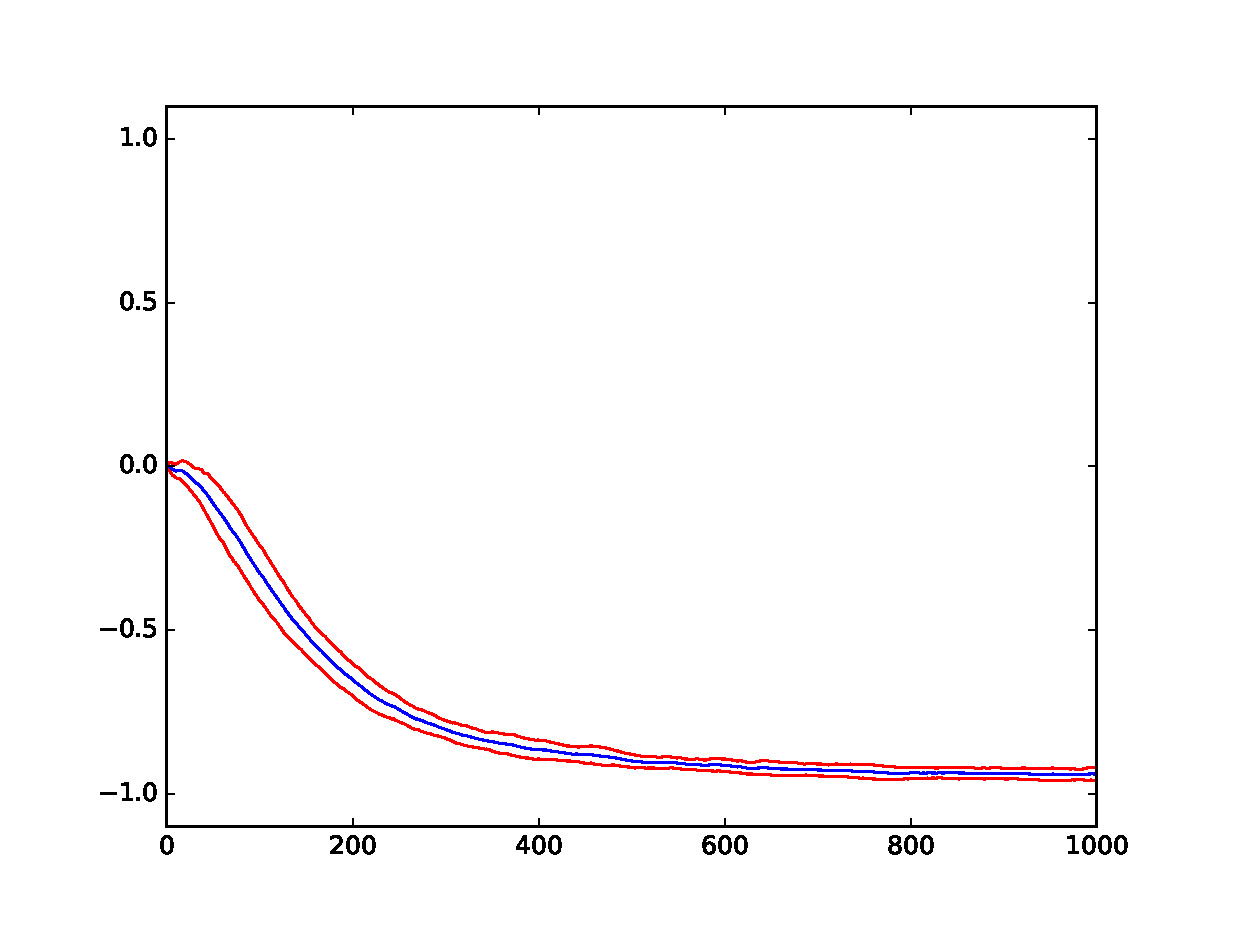
\includegraphics[width=.9\linewidth]{00_00_Q}
	\caption{\textcolor{red}{$\alpha=0$, $\beta=0$}. Average trajectory of defect-cooperate ratio over 50 IPD games and variances. +1 represent a full cooperation (both agents cooperate) and -1 represent a full defection (both agents defect). the trajectory is computed with an exponential moving average of this ratio.}
	\label{00_00_Q}
	%\vskip -6pt
\end{figure}

\subsection{Q-learning with empathy \& gratitude}\label{62}

\textbf{Gentle vs gentle}: Here we look at the behavior of agents where both receive positive intrinsic reward for empathy and gratitude ($\alpha=0.9$, $\beta=0.3$). Paradoxically, it sped up Nash equilibrium's attraction (see figure~\ref{90_90_Q}). As in pure Q-learning situation, both agents learned a false reward function where $\mathcal{P}$ is hight for the other (see column $\mathcal{P}$ of table~\ref{R_90_90_Q}). Indeed, they were intrinsically rewarded by empathy while they where defecting. Furthermore, as they also learned that the other is punished while they both cooperate (see column $\mathcal{R}$ of table~\ref{R_90_90_Q}), they where intrinsically punished while they cooperated. 

\begin{table}[h]
	\centering
	\begin{tabular}{|c|c|c|c|c|} \hline
		&$\mathcal{T}$&$\mathcal{R}$&$\mathcal{P}$&$\mathcal{S}$\\ \hline
		Truth & 1 &  \cellcolor{yellow!30}0.6 & \cellcolor{yellow!30}0 & -1\\ \hline \hline
		$\hat R_{1:2}$ &  0.39 &  \cellcolor{yellow!30}-0.28 &  \cellcolor{yellow!30}1.     &    -0.69\\ \hline
		$\sigma^2$ &  1.9e-01 &   \cellcolor{yellow!30}2.2e-01 & \cellcolor{yellow!30} 1.7e-27  & 7.8e-02\\ \hline \hline
		$\hat R_{2:1}$ & 0.56&  \cellcolor{yellow!30}-0.32 & \cellcolor{yellow!30}0.99& -0.62\\ \hline
		$\sigma^2$ & 1.6e-01  &  \cellcolor{yellow!30}2.5e-01  & \cellcolor{yellow!30}7.7e-08 &  9.6e-02\\ \hline
	\end{tabular}
	\caption{\textcolor{red}{$\alpha=0.9$, $\beta=0.3$}. Average learned other's rewards functions by agents 1 and 2 over 50 IPD games and variances. We can see that with a small variance agents successfully learned that the other has negative reward $\mathcal{S}$, but as the other was always defecting at the end, both thought that the other had strong positive reward $\mathcal{P}$ that is, in fact, null. Furthermore, as they also learned that the other is punished while they both cooperate and receive reward $\mathcal{R}$ (see yellow cells).}
	\label{R_90_90_Q}
\end{table}

\begin{figure}[h]
	\centering
	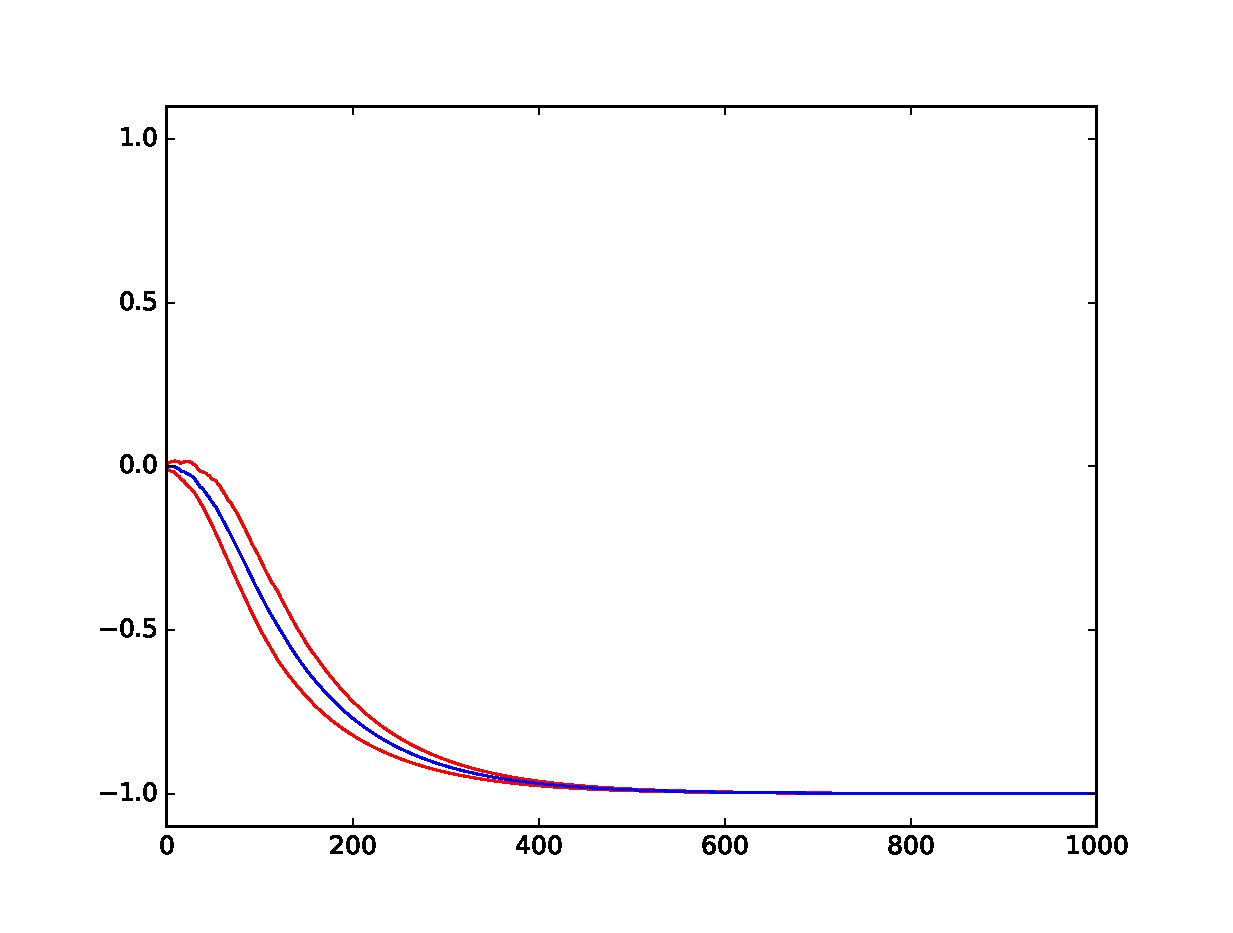
\includegraphics[width=.9\linewidth]{90_90_Q}
	\caption{\textcolor{red}{$\alpha=0.9$, $\beta=0.3$}. Average trajectory of defect-cooperate ratio over 50 IPD games and variances. +1 represent a full cooperation (both agents cooperate) and -1 represent a full defection (both agents defect). the trajectory is computed with an exponential moving average of this ratio.}
	\label{90_90_Q}
	%\vskip -6pt
\end{figure}


\textbf{Aggressive vs aggressive}: This time we looked at the opposite situation, where both agents were intrinsically punished by empathy or gratitude ($\alpha= -0.9$, $\beta= -0.3$). Again paradoxically, it slowed down Nash equilibrium's attraction (see figure~\ref{m9_m9_Q}). For the same reason: since both agent learned the other is rewarded by $\mathcal{P}$, they were intrinsically punished when they defected while the other was cooperating (see column $\mathcal{P}$ of table~\ref{R_m9_m9_Q}).

\begin{table}[h]
	\centering
	\begin{tabular}{|c|c|c|c|c|} \hline
		&$\mathcal{T}$&$\mathcal{R}$&$\mathcal{P}$&$\mathcal{S}$\\ \hline
		Truth & 1 & 0.6 & \cellcolor{yellow!30}0 & -1\\ \hline \hline
		$\hat R_{1:2}$ &  0.79 &-0.23 & \cellcolor{yellow!30}0.58& -0.41\\ \hline
		$\sigma^2$ &   0.073 &  0.14& \cellcolor{yellow!30}0.16 &  0.089\\ \hline \hline
		$\hat R_{2:1}$ & 0.65 &-0.16&\cellcolor{yellow!30} 0.55 & -0.37\\ \hline
		$\sigma^2$ & 0.14 & 0.16 & \cellcolor{yellow!30}0.15  &  0.083\\ \hline
	\end{tabular}
	\caption{\textcolor{red}{$\alpha=-0.9$, $\beta = -0.3$}. Average learned other's rewards functions by agents 1 and 2 over 50 IPD games and variances. We can see that with a small variance agents successfully learned that the other has negative reward $\mathcal{S}$, but as the other was always defecting at the end, both thought that the other had strong positive reward $\mathcal{P}$ that is, in fact, null (see yellow cells).}
	\label{R_m9_m9_Q}
\end{table}

\begin{figure}[h]
	\centering
	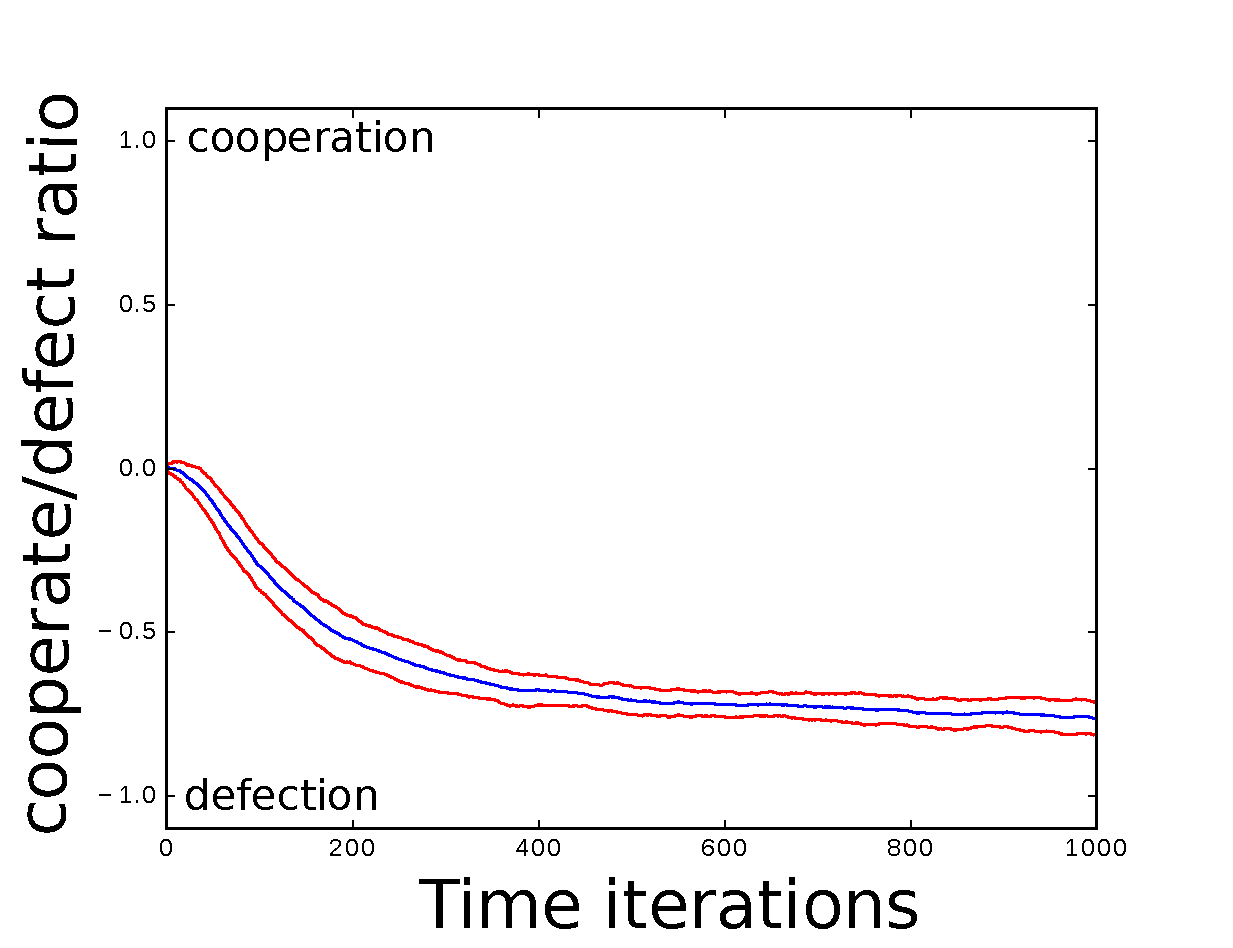
\includegraphics[width=.9\linewidth]{m9_m3_Q}
	\caption{\textcolor{red}{$\alpha=-0.9$, $\beta=-0.3$}. Average trajectory of defect-cooperate ratio over 50 IPD games and variances. +1 represent a full cooperation (both agents cooperate) and -1 represent a full defection (both agents defect). the trajectory is computed with an exponential moving average of this ratio.}
	\label{m9_m9_Q}
	%\vskip -6pt
\end{figure}


\subsection{Expressing intentions with empathy \& gratitude}\label{63}
Here we implemented the expressing-intentions behavior described in section~\ref{3}. The choice of the threshold $\theta$ that determines if the previous reward was worth to repeat the previous action is tricky in the case of IPD. If $\mathcal{P}<\theta\leq\mathcal{R}$ , then agents always cooperate. Indeed, as soon as both agents defect, they simultaneously change to cooperation and keep cooperating till the end. For a similar reason, if $\mathcal{P}\geq\theta$, then, if both agents start by cooperation, they always cooperate otherwise they always defect. In both cases, they can not efficiently learn the reward function of the other. This singularity comes from the fact agents just have two possibilities of action. To avoid this problem, we used a random threshold $\theta$ that is, with probability $p=\mathcal{R}$, higher than $\mathcal{R}$ and with probability $1-p$ smaller than $\mathcal{R}$ (which amounts, in our case, to take $\theta$ uniformly in [0;1]). In a sens, this stochastic choice represents the hesitation of agents between two temptations: to be content with $\mathcal{R}$ or to focus on maximal reward $\mathcal{T}$. 

In our simulations, at the beginning (from $t=0$ up to $t=300$) both agents are following Q-learning behavior. Then, during a phase (from $t=301$ up to $t=700$) they express their intentions using the algorithm of section~\ref{3}. Finally, assuming they had time to learn about each other, they move back to Q-learning till the end (from $t=701$ up to $t=1000$).

\textbf{Only empathy}: we first look at the resulting behavior when both agents just receive intrinsic reward for empathy ($\alpha=0.9$, $\beta=0$). As a result, at the beginning agents were attracted by Nash equilibrium. Then, while they were expressing their intentions, in average they defected as much as they cooperated. After this expressing phase, agent could better understand each other's intentions (see table~\ref{R_90_90_B}) and, led by intrinsic reward for empathy, they started to always cooperate (see figure~\ref{90_90_B}).
\begin{table}[h]
	\centering
	\begin{tabular}{|c|c|c|c|c|} \hline
		&$\mathcal{T}$&$\mathcal{R}$&$\mathcal{P}$&$\mathcal{S}$\\ \hline
		Truth & \cellcolor{yellow!30}1 & \cellcolor{yellow!30}0.6 & 0 & -1\\ \hline \hline
		$\hat R_{1:2}$ & \cellcolor{yellow!30} 0.56&  \cellcolor{yellow!30}0.99& -0.92 &-0.68\\ \hline
		$\sigma^2$ &  \cellcolor{yellow!30}7.6e-02  & \cellcolor{yellow!30}3.0e-09  & 9.1e-02 &  1.0e-01\\ \hline \hline
		$\hat R_{2:1}$ & \cellcolor{yellow!30}0.54 & \cellcolor{yellow!30}0.99& -0.88& -0.72\\ \hline
		$\sigma^2$ & \cellcolor{yellow!30}9.3e-02&   \cellcolor{yellow!30}4.6e-10 &  9.5e-02 &  9.3e-02\\ \hline
	\end{tabular}
	\caption{\textcolor{red}{$\alpha=0.9$, $\beta = 0$}. Average learned other's rewards functions by agents 1 and 2 over 50 IPD games and variances. Between times $t=301$ and $t=700$ agents were following expressing-intention behavior. Agents could learn each other's intentions and understood that $\mathcal{T}$ and $\mathcal{R}$ are positive rewards for the other. As they finally always cooperated (because of empathy), they estimated other's rewards higher for $\mathcal{R}$ than for $\mathcal{T}$(see yellow cells).}
	\label{R_90_90_B}
\end{table}

\begin{figure}[h]
	\centering
	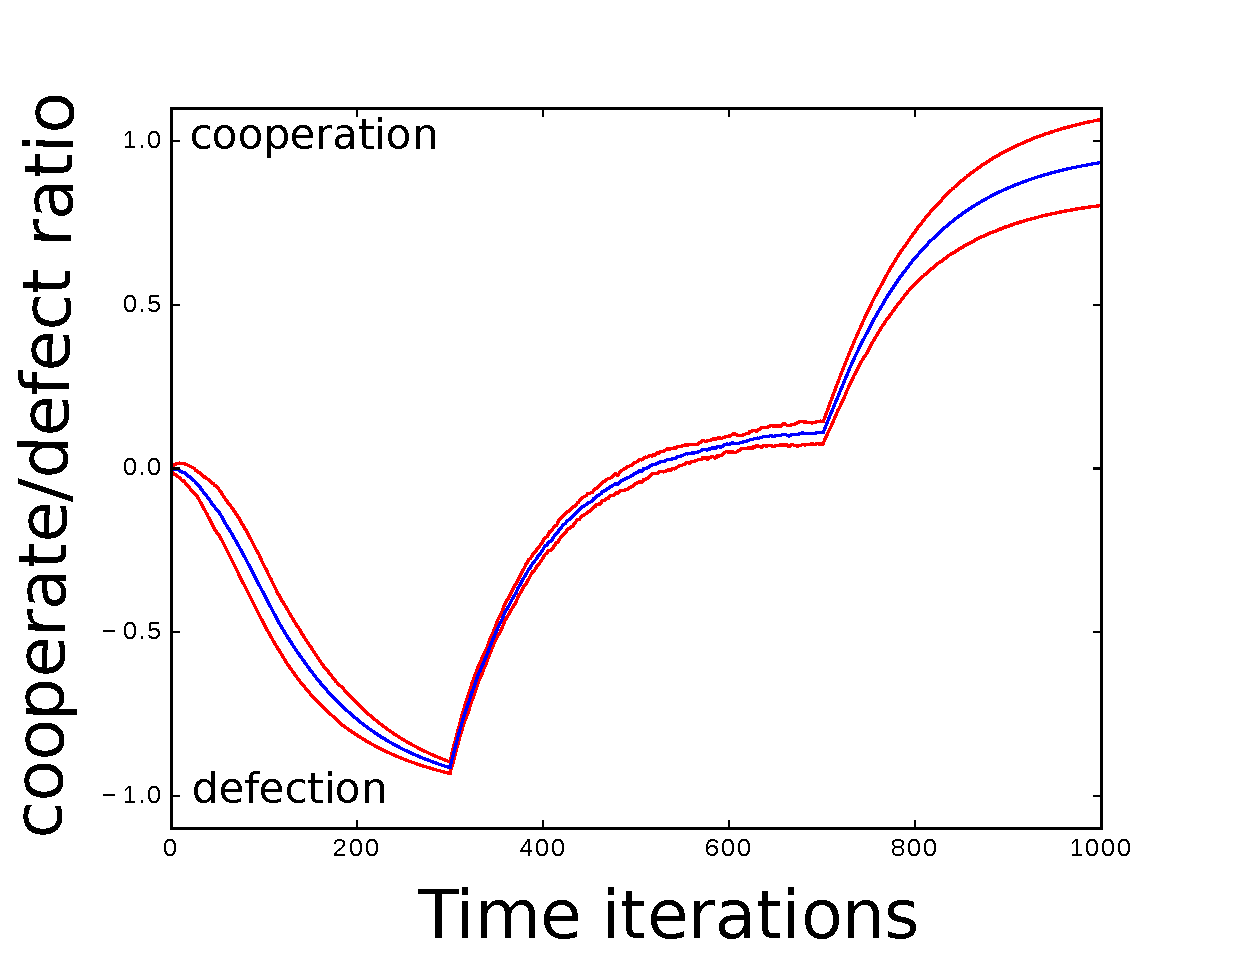
\includegraphics[width=.9\linewidth]{90_90_B}
	\caption{\textcolor{red}{$\alpha=0.9$, $\beta=0$}. Average trajectory of defect-cooperate ratio over 50 IPD games and variances. +1 represent a full cooperation (both agents cooperate) and -1 represent a full defection (both agents defect). the trajectory is computed with an exponential moving average of this ratio. Between times $t=301$ and $t=700$ agents were following expressing-intention behavior.}
	\label{90_90_B}
	%\vskip -6pt
\end{figure}

\textbf{Only Gratitude}: this time both agents just receive intrinsic reward for gratitude ($\alpha=0.$, $\beta=0.9$). As a result, at the beginning agents were attracted by Nash equilibrium. Then, while they were expressing their intentions, they defected as much as they cooperated in average. After this expressing phase, agent could not understand each other's intentions (see table~\ref{R_09_09_B}) and although led by gratitude, they started to always defect (see figure~\ref{09_09_B}).

\begin{table}[h]
	\centering
	\begin{tabular}{|c|c|c|c|c|} \hline
		&$\mathcal{T}$&$\mathcal{R}$&$\mathcal{P}$&$\mathcal{S}$\\ \hline
		Truth & 1 & 0.6 & \cellcolor{yellow!30}0 & -1\\ \hline \hline
		$\hat R_{1:2}$ &  0.58& -0.068 & \cellcolor{yellow!30} 0.99 &-0.68\\ \hline
		$\sigma^2$ &  5.3e-02 &  6.9e-02 & \cellcolor{yellow!30} 3.9e-07 &  3.9e-02\\ \hline \hline
		$\hat R_{2:1}$ & 0.58 &-0.064 & \cellcolor{yellow!30}0.99& -0.66\\ \hline
		$\sigma^2$ &  0.034 & 0.095 & \cellcolor{yellow!30}8.5e-4  & 0.034\\ \hline
	\end{tabular}
	\caption{\textcolor{red}{$\alpha=0$, $\beta = 0.9$}. Average learned other's rewards functions by agents 1 and 2 over 50 IPD games and variances. Between times $t=301$ and $t=700$ agents were following expressing-intention behavior. We can see that with a small variance agents successfully learned that the other has negative reward $\mathcal{S}$, but as the other was always defecting at the end, both thought that the other had strong positive reward $\mathcal{P}$ that is, in fact, null (see yellow cells)}
	\label{R_09_09_B}
\end{table}


\begin{figure}[h]
	\centering
	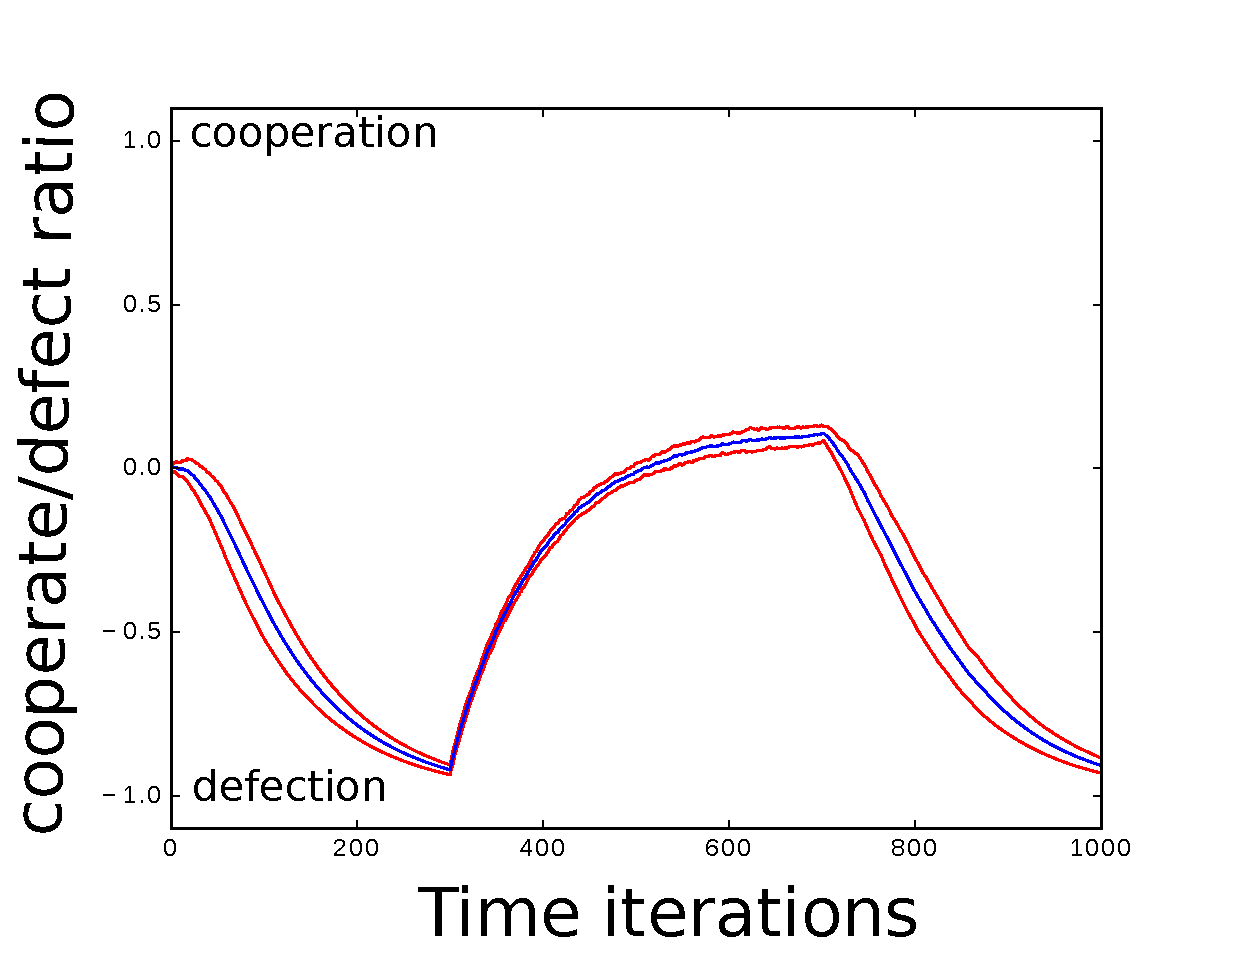
\includegraphics[width=.9\linewidth]{09_09_B}
	\caption{\textcolor{red}{$\alpha=0$, $\beta=0.9$}. Average trajectory of defect-cooperate ratio over 50 IPD games and variances. +1 represent a full cooperation (both agents cooperate) and -1 represent a full defection (both agents defect). the trajectory is computed with an exponential moving average of this ratio. Between times $t=301$ and $t=700$ agents were following expressing-intention behavior.}
	\label{09_09_B}
	%\vskip -6pt
\end{figure}

\textbf{Empathy and gratitude}: Finally we look at the resulting behavior when both agents receive intrinsic rewards for both empathy and gratitude ($\alpha=0.9$, $\beta=0.3$). Like in only-empathy condition, agents successfully understood each other's intentions (see table~\ref{R_99_99_B}). But adding the intrinsic reward for gratitude sped up the cooperation after the expressing-intention phase, increasing the frequency of double cooperation (see figure~\ref{99_99_B}).

\begin{table}[h]
	\centering
	\begin{tabular}{|c|c|c|c|c|} \hline
		&$\mathcal{T}$&$\mathcal{R}$&$\mathcal{P}$&$\mathcal{S}$\\ \hline
		Truth & \cellcolor{yellow!30}1 & \cellcolor{yellow!30}0.6 & 0 & -1\\ \hline \hline
		$\hat R_{1:2}$ & \cellcolor{yellow!30}0.62 &  \cellcolor{yellow!30}1.   &      -0.95& -0.7\\ \hline
		$\sigma^2$ &  \cellcolor{yellow!30}7.0e-02  & \cellcolor{yellow!30}1.8e-17 &  1.4e-02 &  8.6e-02\\ \hline \hline
		$\hat R_{2:1}$ &\cellcolor{yellow!30}0.55 & \cellcolor{yellow!30}1.    &     -0.933 &-0.77\\ \hline
		$\sigma^2$ &  \cellcolor{yellow!30}7.7e-02 &  \cellcolor{yellow!30}1.9e-17  & 2.2e-02  & 7.4e-02\\ \hline
	\end{tabular}
	\caption{\textcolor{red}{$\alpha=0.9$, $\beta = 0.3$}. Average learned other's rewards functions by agents 1 and 2 over 50 IPD games and variances. Between times $t=301$ and $t=700$ agents were following expressing-intention behavior. Agents could learn each other's intentions and understood that $\mathcal{T}$ and $\mathcal{R}$ are positive rewards for the other. As they finally always cooperated (because of empathy), they estimated other's rewards higher for $\mathcal{R}$ than for $\mathcal{T}$(see yellow cells).}
	\label{R_99_99_B}
\end{table}

\begin{figure}[h]
	\centering
	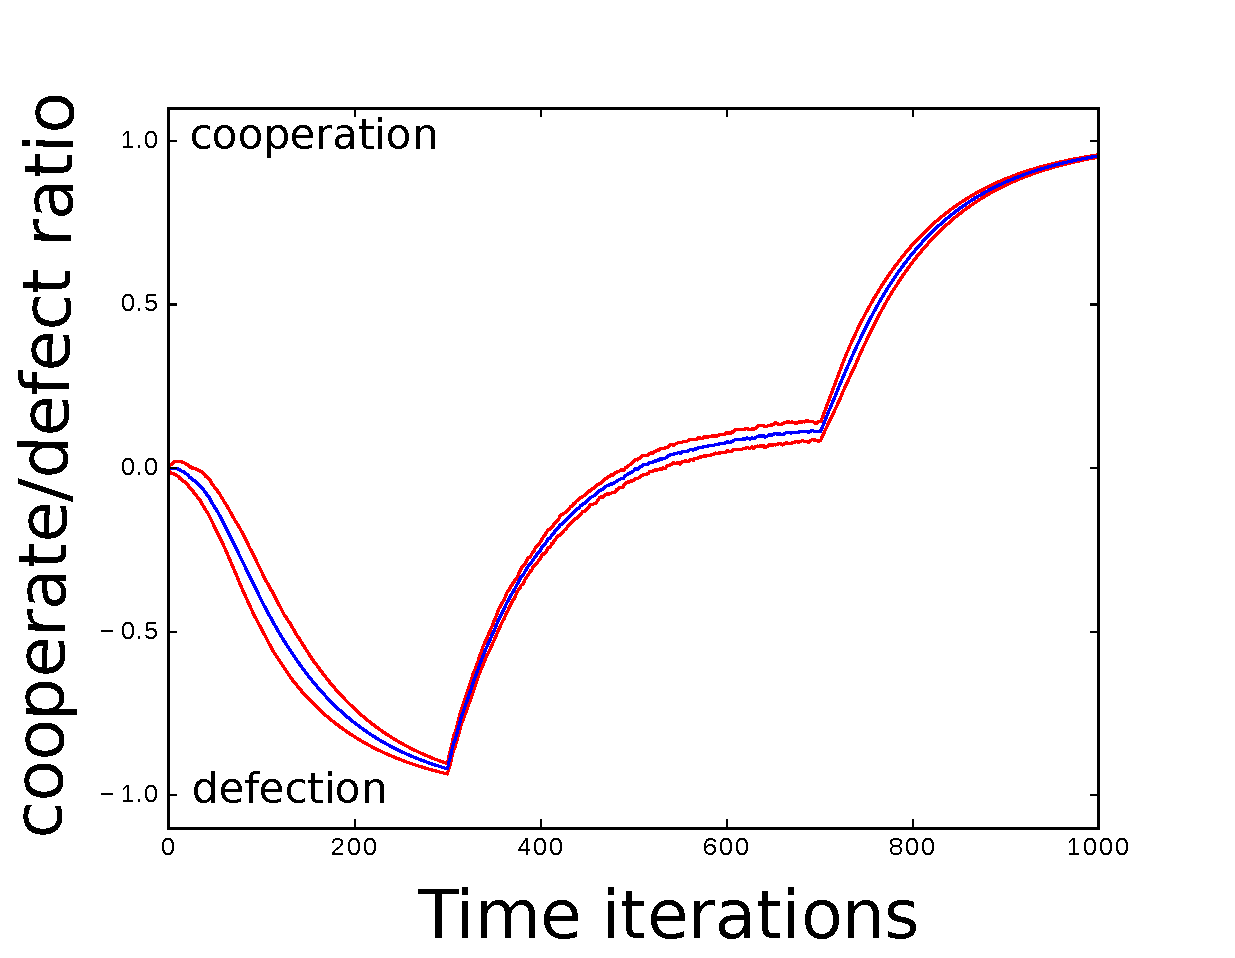
\includegraphics[width=.9\linewidth]{99_99_B}
	\caption{\textcolor{red}{$\alpha=0.9$, $\beta=0.3$}. Average trajectory of defect-cooperate ratio over 50 IPD games and variances. +1 represent a full cooperation (both agents cooperate) and -1 represent a full defection (both agents defect). the trajectory is computed with an exponential moving average of this ratio. Between times $t=301$ and $t=700$ agents were following expressing-intention behavior.}
	\label{99_99_B}
	%\vskip -6pt
\end{figure}


\subsection{Playing with empathy}

Regarding results of subsection~\ref{63} it appears that with expressing-intention phases, empathy is a necessary and sufficient condition to reach cooperation, while gratitude added to empathy stabilizes this cooperation. This is why we finally focused just on empathy in order to explore all possible combination of the $\alpha$ parameters of both agents ($\alpha_1$ for agent 1, $\alpha_2$ for agent 2). For that, we divided the area of possible values in a grid of 20 values between -1 and 1 for both parameters $\alpha$. We simulated 10 IDP games with an expressing intention phase for each of the 400 resulting combinations. We displayed the average final defect-cooperate ratio (the same measure used for all figure in the previous subsection) on a map reported in figure~\ref{alphamap}. We can see that cooperation only occurs when both agents have an higher enough intrinsic reward for empathy ($\alpha>\sim 0.5$ in this case). Interestingly, at the edge between cooperations and Nash equilibrium's defections, appears a balanced zone, where agents equally defect or cooperate (see green area on figure~\ref{alphamap}).

\begin{figure}[h]
	\centering
	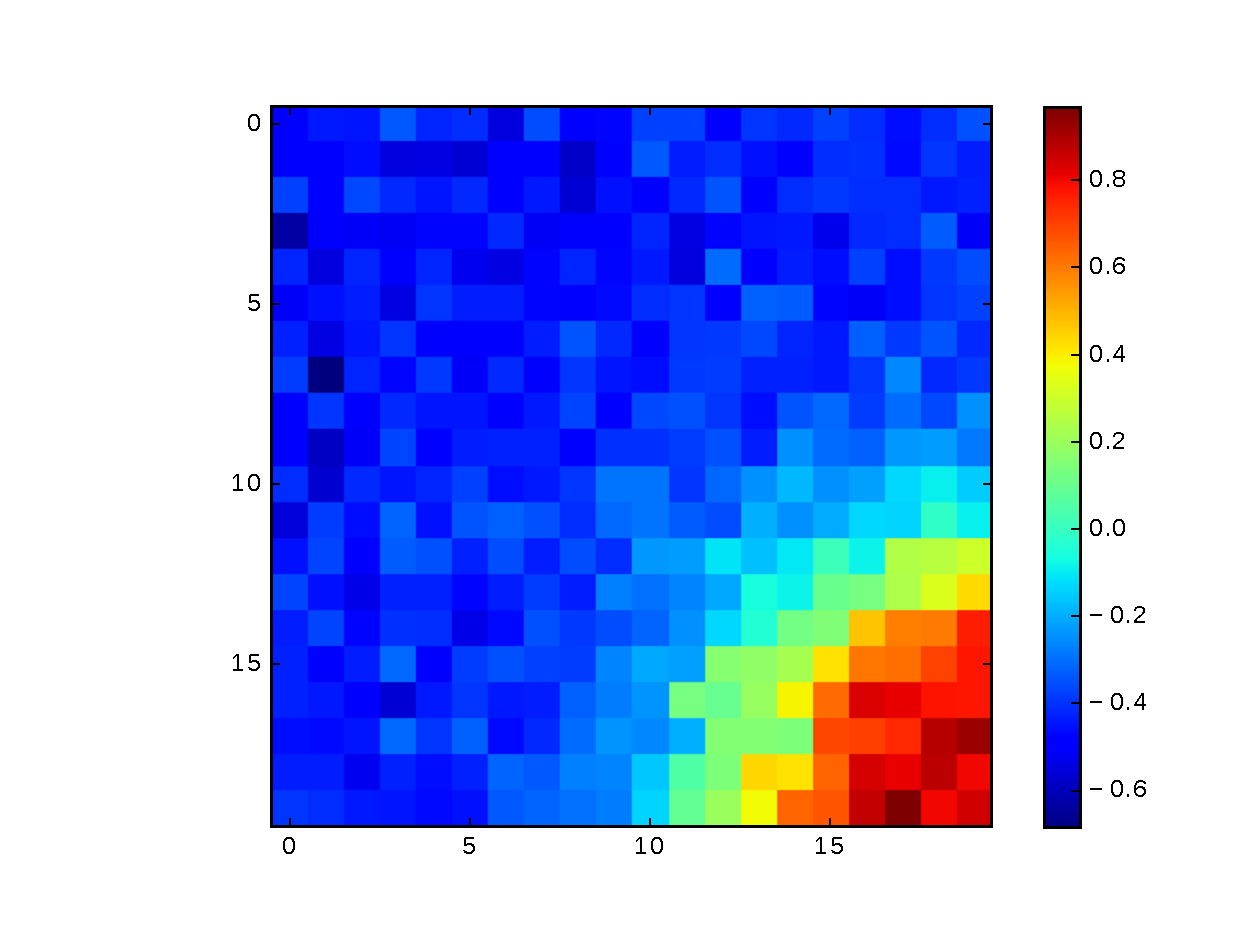
\includegraphics[width=.9\linewidth]{alphamap}
	\caption{Average final defect-cooperate ratio over 10 IDP games for a grid of 400 possible ($\alpha_1$, $\alpha_2$) combinations. In each game, agents were following expressing-intention behavior between time $t=301$ and $t=700$. Red areas correspond to combinations that led to cooperation while blue areas correspond to combinations that led to Nash equilibrium. In green areas, agents where equally defecting and cooperating.}
	\label{alphamap}
	%\vskip -6pt
\end{figure}

\section{Conclusion}

Cooperation in IPD game is said to be irrational. Regarding animals and humans behaviors, we can however observe quantities of such irrational behaviors emerging out of a stressful word, such as friendship or love. Models of natural selection brought global explanations of these emergences, but the detailed causes and mechanisms leading to such complex abilities in animals remain unknown. We strongly believe that any social behavior springs up in such conditions it was rational to behave that way. With this work, we claim that cooperation is no more irrational when agents can express and understand each others intentions. 

We introduce a cognitive architecture enabling second order of theory of mind for social agents. This architecture is not recursive in the sens that each agent develop models for itself, others or itself perceived by others and none of these models enable theory of mind. Agents are modeled as RL-agents and use IRL to model others or themselves seen by others. In this framework, it is possible to design a decision making algorithm aiming to enable agents to express each others intentions. We add two intrinsic rewards based on empathy and gratitude, empathy being the ability to feel others rewards while gratitude is to feel how others would estimate agents own rewards. Through an 2-agents system based on IPD game, we show that when agents can express their intentions, the intrinsic reward for empathy is a necessary and sufficient condition to promote cooperation, while gratitude added to empathy seems to speed up and stabilize this cooperation. 

We make the assumption that our algorithm used to express intentions could also work with humans and hence improve Human-Robot interactions, especially in cooperative tasks. We finally invite readers of this work to explore the huge area of possibilities opened by this framework, by trying different learning approaches, intrinsic rewards and multi-agent scenarios. 


\bibliographystyle{abbrv}
\bibliography{biblio}  
% sigproc.bib is the name of the Bibliography in this case
% You must have a proper ".bib" file
%  and remember to run:
% latex bibtex latex latex
% to resolve all references
%
% ACM needs 'a single self-contained file'!
%\balancecolumns % GM June 2007
% That's all folks!
\end{document}
